\documentclass[11pt]{article}

\usepackage[a4paper,hmargin=2.8cm,vmargin=2.4cm]{geometry}
\usepackage{titlesec}
\usepackage{mathtools}
\usepackage{listings}

\usepackage{graphicx}

\usepackage{biblatex}
\usepackage{hyperref}
\usepackage{cleveref}

\bibliography{tp2refs}

%% Set title

\title{\textit{Algorithms for speech and language processing}\\
{\sffamily TP2 Report: \textit{Building a probabilistic parser for French}}}

\author{Wilson Jallet}

\titleformat{\section}[hang]{\LARGE\bfseries\sffamily}{\thesection}{.5em}{}[]
\titleformat{\paragraph}[hang]{\large\bfseries\sffamily}{}{1em}{}[]

%% Set commands

\newcommand{\calN}{\mathcal{N}}
\newcommand{\calO}{\mathcal{O}}

\newcommand{\wer}{\mathrm{WER}}


\lstset{
	basicstyle=\sffamily,
	stringstyle=\sffamily,
	language=Python}

\begin{document}
\maketitle

\section{Implementation}

\paragraph{Building the PCFG and lexicon}

We use the Python Natural Language ToolKit (NLTK) \cite{nltkCitation} package to parse the treebank data as constituency trees. These trees are then shuffled together before splitting between training, development and testing data. This is needed because lines in the treebank seem to be grouped together thematically\footnote{For instance l. 800--1000 discuss health, and l. 2700--2800 seem to discuss French politics.}. For reproducibility, we fixed the value of the random seed.

We then strip the lexical rules, leaving the part-of-speech (PoS) as terminals, and build the PCFG from these productions using NLTK's PCFG data structure and a helper which computes the empirical probabilities of individual productions.

The lexical rules are transformed into a lexicon using our own \lstinline|ProbabilisticLexicon| Python class, which uses the NLTK probabilistic production data structure to represent the $(\mathrm{token}, \mathrm{PoS}, \mathrm{probability})$ triple.



\paragraph{Out-of-Vocabulary module}

There are two complementary strategies to propose surrogates for out-of-vocabulary (OOV) words: computing \textbf{spelling} nearest neighbors in the corpus according to the Levenshtein Edit distance, and computing \textbf{semantic} nearest neighbors according to the cosine distance of some embeddings (and intersecting with the corpus vocabulary).

For the Levenshtein-nearest neighbors, we run through the corpus and compute all the distances, and get the $k$ elements with the lowest distance (without sorting).
For the embedding nearest neighbors, we use Scikit-Learn's nearest neighbors implementation \cite{scikit-learn} (which is very efficient), which we fit using the cosine distance to measure semantic similarity\footnote{We actually use the Euclidean distance on normalized embedding vectors, which is equivalent to the cosine distance because $\|\frac{x}{\|x\|} - \frac{y}{\|y\|}\|^2 = 2 - 2\langle \frac{x}{\|x\|}, \frac{y}{\|y\|}\rangle$.}.

In order to score the combined list of proposals, we use a language model trained on the corpus. We use NLTK's language modeling API to extract unigrams and bigrams from the corpus and assign appropriate weighted scores (averaging between bigram and unigram scores).

\section{Results}

Handling OOV proper nouns is a difficult problem, especially when they are the first token in a sentence and thus have no context for the OOV module to use: it happens that common nouns or even verbs are used as replacements when they are picked up by edit distance, see \cref{fig:npParseFailure_didiersoulage}.

\begin{figure}[h]
	\centering
	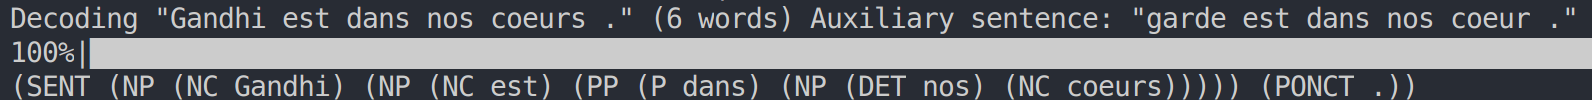
\includegraphics[width=\linewidth]{gandhi-garde.png}
	\caption{Failure of parsing a proper noun which is out-of-vocabulary.}
	\label{fig:npParseFailure_didiersoulage}
\end{figure}


\printbibliography{}


\end{document}